\documentclass[tikz,border=8pt]{standalone}
\usepackage{amsmath}
\usepackage{pgfplots}
\pgfplotsset{compat=1.18}
\definecolor{ink}{HTML}{21352F}
\definecolor{teal}{HTML}{087F7B}
\definecolor{blue}{HTML}{4B77A8}
\definecolor{gold}{HTML}{C58B2A}
\definecolor{rose}{HTML}{B65A62}
\begin{document}
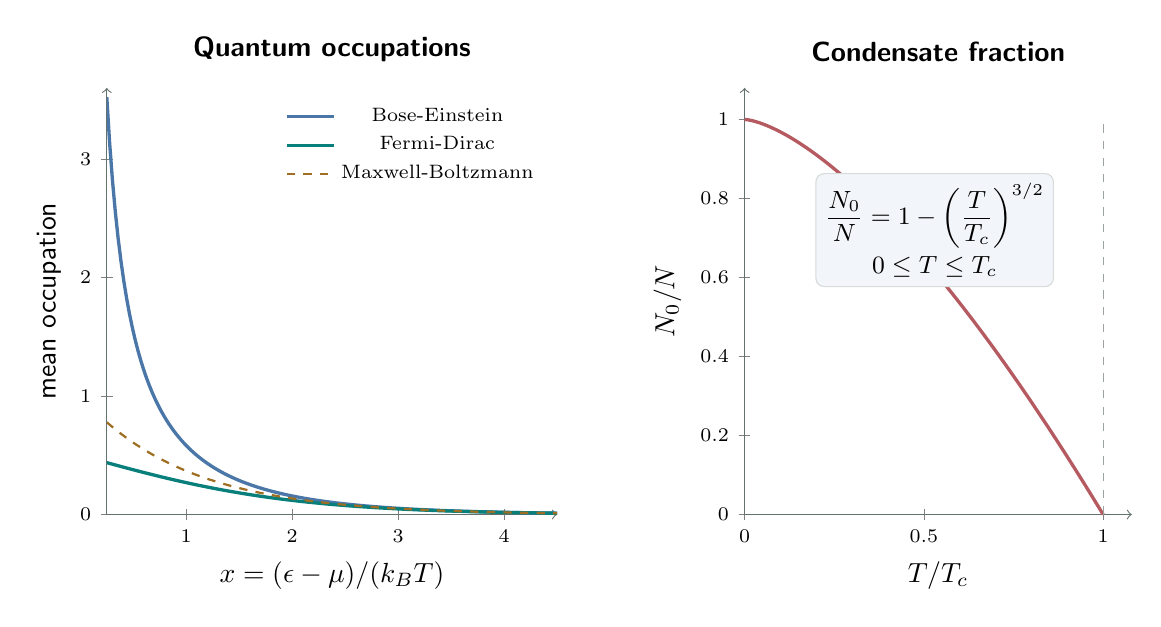
\begin{tikzpicture}[font=\sffamily]
  \begin{axis}[
    at={(0cm,0cm)},anchor=south west,
    width=7.3cm,height=7.0cm,
    xmin=.25,xmax=4.5,ymin=0,ymax=3.6,
    axis lines=left,
    axis line style={draw=ink!70,->},
    xlabel={$x=(\epsilon-\mu)/(k_BT)$},
    ylabel={mean occupation},
    title={\bfseries Quantum occupations},
    legend style={draw=none,fill=none,font=\scriptsize,
      at={(.98,.98)},anchor=north east},
    tick label style={font=\scriptsize}
  ]
    \addplot[blue,very thick,domain=.25:4.5,samples=160]
      {1/(exp(x)-1)};
    \addlegendentry{Bose-Einstein}
    \addplot[teal,very thick,domain=.25:4.5,samples=160]
      {1/(exp(x)+1)};
    \addlegendentry{Fermi-Dirac}
    \addplot[gold!80!black,thick,dashed,domain=.25:4.5,samples=160]
      {exp(-x)};
    \addlegendentry{Maxwell-Boltzmann}
  \end{axis}

  \begin{axis}[
    at={(8.1cm,0cm)},anchor=south west,
    width=6.5cm,height=7.0cm,
    xmin=0,xmax=1.08,ymin=0,ymax=1.08,
    axis lines=left,
    axis line style={draw=ink!70,->},
    xlabel={$T/T_c$},
    ylabel={$N_0/N$},
    title={\bfseries Condensate fraction},
    tick label style={font=\scriptsize},
    clip=false
  ]
    \addplot[rose,very thick,domain=0:1,samples=160]
      {1-x^1.5};
    \addplot[ink!45,dashed] coordinates {(1,0) (1,1)};
    \node[draw=ink!18,fill=blue!7,rounded corners=3pt,
          font=\small,align=center] at (axis cs:.53,.72)
      {$\displaystyle\frac{N_0}{N}
        =1-\left(\frac{T}{T_c}\right)^{3/2}$\\[2pt]
       $0\le T\le T_c$};
  \end{axis}
\end{tikzpicture}
\end{document}
